\documentclass[12pt]{article}

\usepackage[utf8]{inputenc}	%%input font setting
\usepackage[T1]{fontenc} 		%%font for automatic recognition of letters with the accent
\usepackage{amsfonts}		%%fonts for the mathematical rendering of formulas
\usepackage{amssymb}
\usepackage{amsmath}
%% CHAPTERS STRUCTURE
\usepackage[english]{babel} %%Set English as main language of the document
\usepackage{hyperref}
\usepackage{pseudocode} % Environment for specifying algorithms in a natural way
\usepackage{graphicx}
\usepackage{siunitx}
\usepackage{systeme}
\usepackage{easyReview} % for \comment, \alert, etc.
\usepackage{subcaption}
\usepackage{xcolor}
\setlength{\parindent}{0pt}



% \graphicspath{{../plotting/}}

\title{Endocytosis analysis}
\author{Pietro Sillano}
\setlength {\marginparwidth }{2cm}
\begin{document}
\maketitle
\tableofcontents

\section{Introduction}
This part follows closely what has been done by the supplementary material of \cite{agudo-canalejoCriticalParticleSizes2015}. 
The code is adapted from \cite{freyMembraneAreaGain2022} and from supplementary materials of \cite{christActiveShapeOscillations2021}.


\begin{figure}[ht]
  \begin{center}
    \begin{subfigure}{0.9\textwidth}
      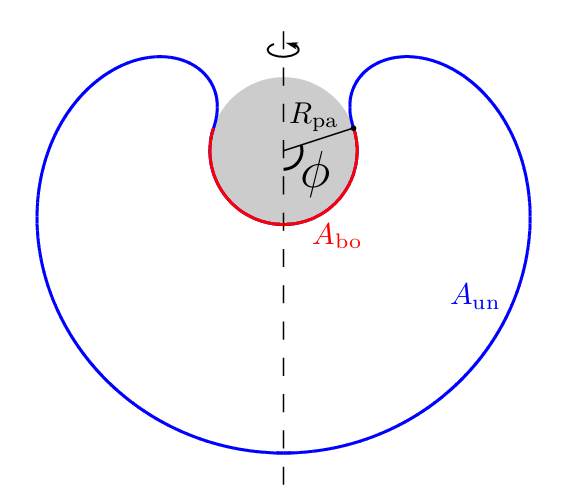
\includegraphics[width=0.45\linewidth]{img/system.png}
      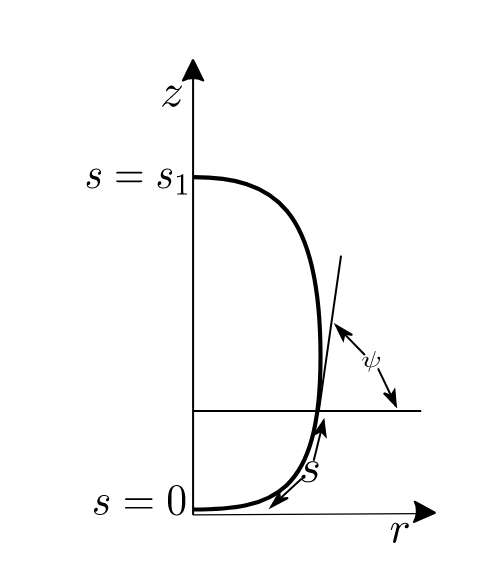
\includegraphics[width=0.45\linewidth]{img/system2.png}
      \caption{image taken from supplementary material of \cite{agudo-canalejoCriticalParticleSizes2015}}
  \end{subfigure}
  \end{center}
  \label{fig:figure1}
\end{figure}

The total free energy of the system will be composed by two contribution representing the bound and unbound segment:

$$
E = E_{bo} + E_{un}
$$

The bound segment of the membrane will follow the particle contour but the unbound segment does not have a trivial shape.

$E_{bo}$ has an adhesive and a bending energy contribution: \cite{agudo-canalejoCriticalParticleSizes2015}
$$
E_{bo} = (-2 \pi |W| R_{pa}^2 + 4 \pi k(1+m R_{pa})^2)(1-\cos \phi) = (-2 \pi |W| R_{pa}^2 + 4 \pi k)(1-\cos \phi)
$$

we are considering a vesicle bilayer with zero spontaneous curvature, ie $m=0$.


In order to find the shape of the unbound segment that minimizes $E_{un}$, for a fixed value of contact angle $\phi$, and satisfies the constraints on the total membrane area $A-A_{bo}$ and enclosed volume $V+V_{bo}$ of the vesicle, we must minimize the shape functional


$$
F = E_{un} + \Sigma(A-A_{bo}) - \Delta P (V+V_{bo}) = \int_{A_{un}} dA \; 2kH^2  + \Sigma(A-A_{bo})
$$

where $\int_{A_{un}} dA \; 2kH^2$ is the Helfrich energy integral.

In our simulations we dont have any control or constraint on the vesicle volume, we dont pay a cost to change the vesicle volume then we put the volume term equal to zero.


Assuming that the vesicle shape will be axis-symmetric around z-axis It is possible to rewrite $F$ in terms of $s,\psi(s),x(s)$:

$$
F = \int_{s_0}^{s^\star} L(s,\psi(s),x(s)) \; ds
$$


The mean curvature $H$ is given by 
$$H=\frac{1}{2}(C_1+C_2)$$

\begin{figure}[ht]
  \begin{center}
      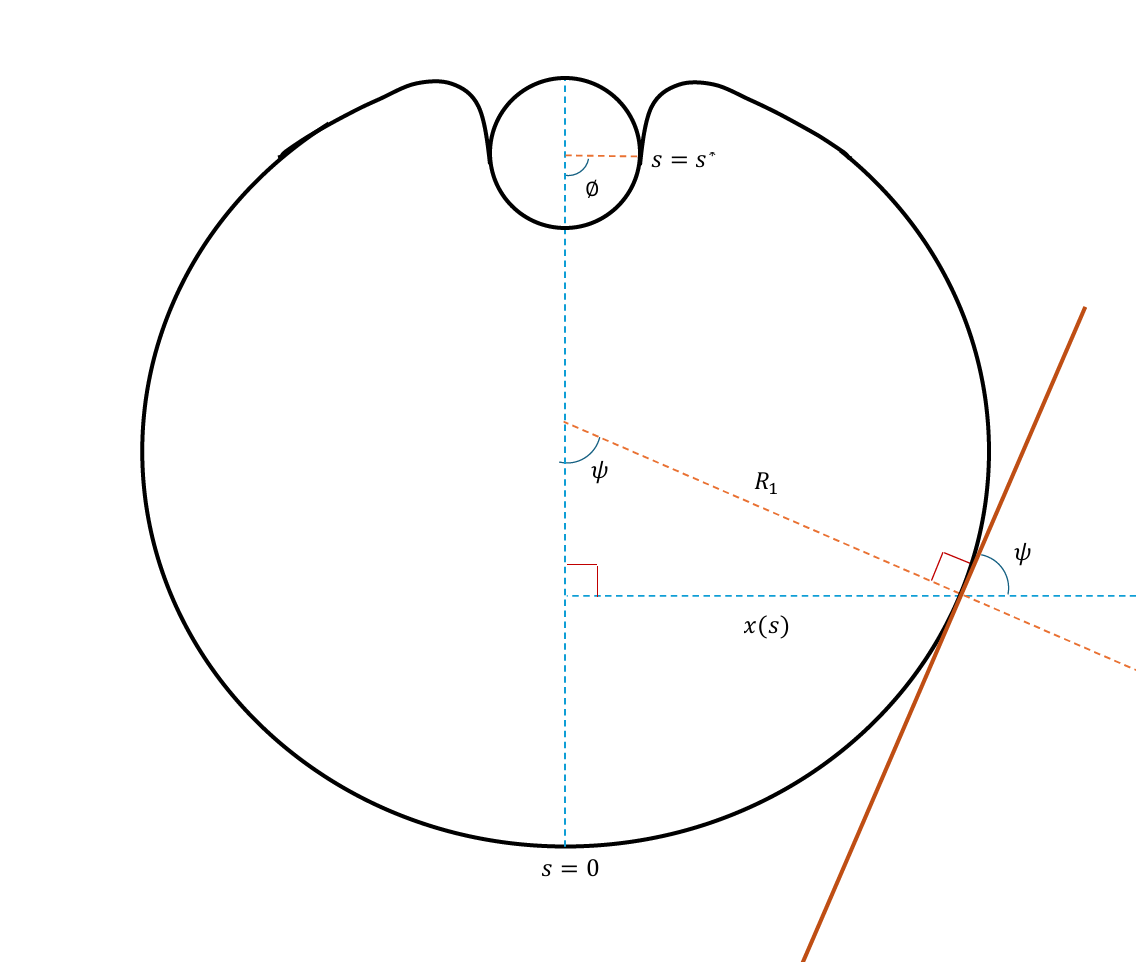
\includegraphics[width=0.8\linewidth]{img/shape_equation_schematic.png}
      \caption{Visualization of the curvature}
  \end{center}
  \label{fig:figure2}
\end{figure}

From figure 2 follows that:
$$
C_1=\frac{1}{R_1}=\frac{\sin{\psi}}{x(s)}
$$

$C_2$ is given by the definition of curvature: the rate at which $\psi$ changes with respect to the arc length $s$, which gives:

$$
C_2=\frac{d\psi}{ds}
$$

\textbf{Note:}  I think that $C_1$ defines the curvature straight into (or out of) the paper, and $C_2$ defines the curvature in the direction of s. 

These two curvatures together give the mean curvature:
$$
H^2=\frac{1}{4}\bigg(\frac{d\psi}{ds}+\frac{\sin{\psi}}{x(s)}\bigg)^2
$$


Now we will parameterize $F$ in terms of $s, \psi(s), x(s)$
$$
F = \int_{A_{un}} dA \; 2kH^2  + \Sigma A_{un} = \int_{s_0}^{s^\star} L(s,\psi(s),x(s)) \; ds
$$


For this step we need to rewrite an integral in terms of $dA$ to an integral in terms of $s$. To do this we use the following formula:
$$
dA=2\pi x(s)ds
$$

applying this formula to $F$ gives:
$$
F = \int_{A_{un}} dA \; 2kH^2  + \Sigma A_{un} = \int_{s_0}^{s^\star} 2\pi x(s)ds \; 2kH^2 + \Sigma \int_{s_0}^{s^\star} 2\pi x(s)  ds
$$

Now we will add the two integrals together and fill in H:
$$
F = 2\pi k \int_{s_0}^{s^\star} \frac{x(s)}{2} \bigg(\dot{\psi}+\frac{\sin{\psi}}{x(s)}\bigg)^2  + \frac{\Sigma}{k} x(s) ds \;
$$

To make sure the relation between $x$ and $\phi$ is satisfied, a Lagrange multiplier is added to the integral.

$$
F = 2\pi k \int_{s_0}^{s^\star} \frac{x(s)}{2} \bigg(\dot{\psi}+\frac{\sin{\psi}}{x(s)}\bigg)^2  + \frac{\Sigma}{k} x(s) +\gamma(\dot{x}-\cos \psi)ds\;
$$

\alert{It is identical to the L that you have except for the k, so maybe I made a mistake somewhere} 


$$
L(s,\psi,\dot{\psi},x,\dot{x},\gamma) = \frac{x}{2} \bigg(\dot{\psi}+\frac{\sin \psi}{x}\bigg)^2 + \Sigma x + \gamma(\dot{x}-\cos \psi)
$$

$\gamma(s)$ is a Lagrange multiplier function that ensure the relation between $x$ and $\psi$ is satisfied.

We want to minimize the functional $F$ using a variational approach $\delta F=0$. $\delta F$ denotes variation with respect to the shape of the vesicle and $\Sigma$ and $P$ are adjusted in order to guarantee the prescribed area and volume. After the minimization you end up with a system of differential equations that once solved it will describe the vesicle shape.

To draw a parallelism it is the same procedure of minimizing the action functional in classical mechanics respect to a trajectory.



\paragraph*{More formally:} 


The solution of the minimization of functional $F$ is given by the Euler-Lagrange equations (see \url{https://en.wikipedia.org/wiki/Euler%E2%80%93Lagrange_equation}). In general, given a functional $I$:
$$I=\int_{x_a}^{x_b}L(x,f_1(x),f_2(x),\dots,\dot{f_1}(x),\dot{f_2}(x),\dots)$$

where $\dot{f_i}(x)=\frac{df_i}{dx}$ the Euler-Lagrange equations are:

$$
\frac{d}{dx}\bigg[ \frac{\partial L}{\partial \dot{f_i}} \bigg] - \frac{\partial L}{\partial f_i} = 0
$$


In our case, the equations will be:
$$
\frac{d}{ds}\bigg[ \frac{\partial L}{\partial \dot{\psi}}(s,\psi,\dot{\psi},x,\dot{x},\gamma) \bigg] - \frac{\partial L}{\partial \psi}(s,\psi,\dot{\psi},x,\dot{x},\gamma) = 0
$$

\paragraph*{Hamiltonian function:}
It is possible to define an "Hamiltonian function":

\begin{equation*}
    H = -L + \dot{\psi} \frac{\partial L}{\partial \dot{\psi}} + \dot{x} \frac{\partial L}{\partial \dot{x}}
    = \frac{x}{2} \bigg[  \dot{\psi}^2 - \frac{\sin \psi}{x}^2 \bigg] - \Sigma x + \gamma \cos \psi
\end{equation*}

$H$ is conserved because $\frac{\partial L}{\partial S} = 0$. It also leads to the boundary condition for $\gamma(s)$ see eqs 3.7 from \cite{seifertShapeTransformationsVesicles1991}.

This Hamiltonian is an "energy" function too.



\subsection{Physical quantity of the system}
The following ones are the physical quantities or the constitutive relations involved in our system of interest:

\begin{itemize}
  \item $R_{pa}$ particle radius
  \item $|W|$ adhesive energy density for area unit
  \item $R_{ve}$ radius of vesicle
  \item $k$ bending rigidity
\end{itemize}

We can describe the system using two adimensional quantity:
$$
r_{pa} = \frac{R_{pa}}{R_{ve}}
$$

$$
w = \frac{|W| R_{pa}^2}{k}
$$

\section{Shape ODE system}
The following is the set of differential equation needed to describe the equilibrium shape of a membrane that interacts with an external particle. This system of equation is:
\begin{itemize}
    \item ordinary because the independent variable is always $\bar{s}$.
    \item First order because all the derivatives are first derivative
    \item Non linear because of non linear terms like squares or trigonometric functions.
    \item it is a system because the dependent variables are coupled.
\end{itemize}


\begin{equation}
  \begin{cases} 
    \frac{d\psi}{ds} =  u \\[3mm]
    \frac{du}{ds} =  [-\frac{u}{x}\cos\psi+\frac{\cos(\psi)\sin(\psi)}{x^2}+\frac{\gamma\sin \psi}{2\pi k x}] \\[3mm]
    \frac{d\gamma}{ds} =  [\pi k (u^2-\frac{\sin^2 \psi}{x^2})+2 \pi \Sigma] \\[3mm]
    \frac{dx}{ds} =  \cos \psi \\[3mm]
  \end{cases}
\end{equation}


It is possible to augment the equation in the systems with two additional odes for area and volume of the vesicle:

\begin{equation}
  \begin{cases}
    \frac{dA}{ds} =  2 \pi x \\[3mm]
    \frac{dV}{ds} = \pi x^2 \sin{\psi}
  \end{cases}
\end{equation}



\subsection{Non-dimensionalization step}
$$
R_{ve} = \sqrt{\frac{A}{4 \pi}}
$$

Given $R_{ve}$ as length scale, $k$ as basic energy scale and $s^\star$ as the bound arc length we can rewrite our equation in a unitless form:

The dash symbols are the unitless quantities.
\alert{write in a better way, maybe in a table}


$$
\bar{\psi} = \psi
$$

$$
\bar{u} = u R_{ve}
$$

$$
\bar{x} = \frac{x}{R_{ve}}
$$

$$
\bar{\gamma} = \gamma R_{ve}
$$

$$
\bar{\Sigma} = \Sigma \frac{R_{ve}^2}{k}
$$

$$
\bar{A} = \frac{A}{4 \pi R_{ve}^2 }
$$

$$
\bar{V} = \frac{3V}{4 \pi R_{ve}^3 }
$$

$$
\bar{s} = \frac{s}{s^\star}
$$

$$
\bar{s^\star} = \frac{s^\star}{s^\star} = 1
$$

$$
\Omega = \frac{s^\star}{R_{ve}}
$$
 

Substitute in the system we get:
\begin{equation}
  \begin{cases} 
    
    \frac{d\bar{\psi}}{d\bar{s}} = \Omega \bar{u} \\[3mm]
    \frac{d\bar{u}}{d\bar{s}} = \Omega [-\frac{\bar{u}}{\bar{x}}\cos\bar{\psi}+\frac{\cos(\bar{\psi})\sin(\bar{\psi})}{\bar{x}^2}+\frac{\bar{\gamma}\sin \bar{\psi}}{2\pi k \bar{x}}] \\[3mm]
    \frac{d\bar{\gamma}}{d\bar{s}} = \Omega [\pi k (\bar{u}^2-\frac{\sin^2 \bar{\psi}}{\bar{x}^2})+2 \pi \bar{\Sigma} k] \\[3mm]
    \frac{d\bar{x}}{d\bar{s}} = \Omega \cos \bar{\psi} \\[3mm]
    \frac{d\bar{A}}{d\bar{s}} = \frac{1}{2}\Omega \bar{x} \\[3mm]
    % \frac{d\bar{V}}{d\bar{s}} = \frac{3}{4}\Omega \bar{x}^2 \sin{\bar{\psi}}
  \end{cases}
\end{equation}

% $$
% \frac{d\bar{\psi}}{d\bar{s}} = \Omega \bar{u}
% $$

% $$
% \frac{d\bar{u}}{d\bar{s}} = \Omega [-\frac{\bar{u}}{\bar{x}}\cos\bar{\psi}+\frac{\cos(\bar{\psi})\sin(\bar{\psi})}{\bar{x}^2}+\frac{\bar{\gamma}\sin \bar{\psi}}{2\pi k \bar{x}}]
% $$

% $$
% \frac{d\bar{\gamma}}{d\bar{s}} = \Omega [\pi k (\bar{u}^2-\frac{\sin^2 \bar{\psi}}{\bar{x}^2})+2 \pi \bar{\Sigma} k]
% $$

% $$
% \frac{d\bar{x}}{d\bar{s}} = \Omega \cos \bar{\psi}
% $$

% $$
% \frac{d\bar{A}}{d\bar{s}} = \Omega \bar{x}
% $$

% $$
% \frac{d\bar{V}}{d\bar{s}} = \frac{3}{4}\Omega \bar{x}^2 \sin{\bar{\psi}}
% $$


\subsection{Initial conditions and parameters}
We ended up with 5 ODEs, we have five boundary conditions at the South Pole ($s=0$):

\alert{Explain why these are zero, especially the gamma }

$$
\psi(s=0)=0, u(s=0)=u_0, \gamma(s=0)=0
$$

$$
x(s=0) = 0, A(s=0)=0
$$

\paragraph*{Explanation of BCs:}
Hamiltonian $H(s=0)=0$ and substituting the value for $\psi,x$ I obtain $\gamma(s=0) \cos(\psi(s=0))=0$ and then $\gamma(s=0)=0$. 

Assuming that $H$ is conserved (\alert{how to verify?}), $H(s=s^\star)=0$ but I cannot solve the system of eq (4 unknwon, 1 equation).

What I get is $$
\gamma^\star=\frac{1}{2} \frac{1}{\cos \psi^\star} \left(\sin ^2 \psi^\star +2 \Sigma x^\star - u_\star^2 x^\star \right)
$$

Probably a good idea is to express $\gamma^\star$ as combination of the other unknowns.

% $$\frac{1}{4} \left(4 \text{gamma} \cos (\text{Psi})+\cos (2 \text{Psi})-4 \text{sigma} x+2 u^2 x-1\right)$$




We also have 5 boundary conditions at the North Pole $s=s^\star$, the first three are known after fixing the contact angle of the particle and the constitutive relations (adhesive energy and bending rigidity) 

$$
\bar{\psi}(s^\star) = \pi + \phi
$$

$$
\bar{x}(s^\star) = \frac{R_{pa}}{R_{ve}} \sin \phi 
$$

$$
\bar{A}(s^\star) = A - A_{bo} = \frac{\bar{A} - \bar{A_{bo}}}{4 \pi R_{ve}^2}
$$

The values of the following two will be part of the free parameters:

$$
\bar{u}(s^\star) = u^\star
$$

$$
\bar{\gamma}(s^\star) = \gamma^\star
$$

where $\bar{A}$ is the total area of vesicle normalized to make it unitless.

\textbf{Oss:} We dont have an equation for the volume because in simulation we are not constraining it and there is no energy cost in changing vesicle internal volume. 
% Therefore, the volume ode will be uncoupled from the others

Then, we have 5 unknown parameters ("randomly" guessed at the beginning of the integration procedure):

$$\Sigma,\; s^\star ,\;u_0,u^\star \text{ and } \gamma^\star$$



\alert{I need to check boundary condition for $\gamma^\star$ and $\gamma_0$ because of the conservation of the Hamiltonian function. Not sure if the condition is satisfied}

\section{Numerical protocol}
\subsection{How (Pietro thinks) it works}
\begin{itemize}
  \item assuming that the constitutive relations of the system $r_{pa}$ and $w$ are given and we know its values.
  \item you will choose a value for $\phi$ the wrapping angle and you will know the $A_{bo}$ \alert{this is actually what concern me more, I would like to include the wrapping angle not as a given parameter!!}
  \item now you have everything to calculate the bound free energy $E_{bo}$
  \item shooting method for the unbound shape: 
    \begin{itemize}
      \item you will start with choosing random free parameters $\Sigma,\; s^\star \text{ and }u_0$
      \item you will integrate the ODE system having the initial conditions for $\psi,u,\gamma,x,A$
      \item after the integration you calculate the residuals as the error between the boundary conditions at $s=s^\star$
      \item the idea is to iterate the integration procedure to minimize the residuals and finding the optimal value of the free parameters.
    \end{itemize}
  \item calculate the total free energy of the system
  \item estabilish if the total free energy is a minimum/stable state for the chosen combination of constitutive relations and contact angle $\phi$.
\end{itemize}


\paragraph{Oss:} the values obtained for the free parameters changes when you change the angle $\phi$. in the same way the free parameters changed in the Felix paper when he changed $m$ and $\nu$.


\section{Expansion at the South pole}

At $s=0$ $x(s)$ goes to zero and it appears as denominator and it leads to divergences causing numerical instability. An easy way to solve this is to regularize the functions at the "South pole" when $s=0$. Regularization means Taylor expansion of all functions around $s=0$.


First you need to expand $x(s),\psi(s),u(s),\gamma(s)$ and substitute the expansion in each equation (both sides) of the system. Then equating the coefficient of the polynomials you can get the series coefficient.

$$
u(s)=u(0) + u_1s + \frac{u_2 }{2}s^2 + \frac{u_3 }{6}s^3 + \frac{u_4 }{24}s^4 + O(s^4)
$$


$$
\cos(\psi(s))= 1 - \frac{\psi(s)^2}{2} + \frac{\psi(s)^4}{24} = 1 - \frac{1}{2} U_0^2 s^2 + \frac{U_0 \psi_2}{2} s^3 + (\frac{psi_2^2}{8} + \frac{U_0 \psi_3}{6}) s^4 +O(s^4);
$$



% $$
% \sin\psi(s)=\frac{\psi_2 s^2}{2}+\frac{1}{6} s^3 
% \psi_3-u_0^3 +\frac{\psi_4 s^4}{24}+s u_0
% $$

% $$
% A(s)=A_1 s+\frac{A_2 s^2}{2}+\frac{A_3 s^3}{6}+\frac{A_4 s^4}{24};
% $$

% $$
% \gamma(s)=\gamma_1 s+\frac{\gamma_2 s^2}{2}+\frac{\gamma_3 s^3}{6}+\frac{\gamma_4 s^4}{24};
% $$

% $$
% V(s)=\frac{s^4 V_4}{24}+\frac{s^3 V_3}{6}+\frac{s^2 V_2}{2}+s V_1;
% $$

% $$
% u(s)=\psi_2 s+\frac{\psi_3 s^2}{2}+\frac{\psi_4 s^3}{6}+\frac{\psi_5 s^4}{24}+u_0;
% $$


% $$
% \frac{d\gamma}{ds}=\gamma_1+\gamma_2 s+\frac{\gamma_3 s^2}{2}+\frac{\gamma_4 s^3}{6}+\frac{\text{gamma5} s^4}{24};
% $$

% $$
% \frac{du}{ds}=\psi_2+\psi_3 s+\frac{\psi_4 s^2}{2}+\frac{\text{psi5} s^3}{6}+\frac{\text{psi6} s^4}{24};
% $$



Considering the simplest (and not trivial) equation from our system $\frac{dx}{ds} =  \cos \psi$ and performing this substitution we'll get the coefficients for $x$ expansion:

$$
x_1 = 1 ,\; x_2 = 0 ,\; x_3 = - u_0^2 ,\; x_4 = 0
$$

$$
x(s)=s-\frac{s^3 u_0^2}{6};
$$

The another equations from the system are quite challenging to deal on pen and paper and for that we have used a Mathematica script to perform the expansion.The final values for the coefficient are:

$$
x_1 = 1 ,\; x_2 = 0 ,\; x_3 = - u_0^2 ,\; x_4 = 0
$$


$$
\psi_1 = u_0  ,\; \psi_2 = 0 ,\; \; \psi_4 = 0
$$
$$
\psi_3 = \frac{3\gamma_1 u_0 - 4 \pi k u_0^3}{2 \pi k } = \frac{6 \pi \Sigma u_0 - 4 \pi k u_0^3}{2 \pi k }
$$


$$
\gamma_1 = 2 \pi \Sigma ,\; \gamma_2 = 0 
$$
$$
\gamma_3 = \frac{4}{3} k \pi \psi_3 u_0 = 4 \pi (\Sigma u_0 - \frac{2}{3} k u_0^3) ,\; \gamma_4 = 0
$$



$$
A_1 = 0 ,\; A_2 =  2 \pi ,\; A_3 = 0 ,\; A_4 = - 2 \pi u_0^2
$$

$$
V_1 = 0 ,\; V_2 = 0 ,\; V_3 = 0 ,\; V_4 = 6 \pi u_0
$$


Then if you want to reconstruct the series:


$$
x(s)=x_1 s+\frac{x_2}{2}s^2+\frac{x_3}{6}s^3+\frac{x_4}{24} s^4 =s-\frac{u_0^2}{6}s^3 
$$

$$
A(s) = \pi s^2 - \frac{\pi u_0^2}{12}s^4
$$


$$
V(s) = \frac{\pi u_0}{4}s^4
$$


$$
\gamma(s) = 2 \pi \Sigma s + \frac{2}{9} k \pi \psi_3 u_0 s^3 = 2 \pi \Sigma s + \frac{1}{9}  u_0 (6 \pi u_0 \Sigma - 4 k u_0^3)s^3
$$

$$
\psi(s)=u_0s + \frac{3  \Sigma u_0 - 2  k u_0^3}{6 k }s^3
$$

$$
u(s)=u(0) + u_1s + \frac{u_2 s^2}{2} + \frac{u_3 s^3}{6} + \frac{u_4 s^4}{24} = u_0 + \psi_2 s + \frac{\psi_3 s^2}{2} + \frac{\psi_4 s^3}{6} + \frac{\psi_5 s^4}{24}
$$

$$
= u_0  + \frac{3  \Sigma u_0 - 2  k u_0^3}{2 k }s^2
$$

This expansions still need to be non-dimensionalized.

\subsection{Non-dimensionalization of the expansion}
Again the dash symbols are the unitless quantities and we applied the same trasformations previously used.


$$
\bar{x_1} = \Omega ,\;  \bar{x_3} = - \Omega^3 \bar{u_0}^2 
$$

$$
\bar{\psi_1}  = \Omega \bar{u_0}
$$

$$
\bar{\psi_3} = (3\bar{\Sigma} \bar{u_0} - 2 \bar{u_0}^3)\Omega^3
$$

$$
\bar{u_0} = \bar{u_0} 
$$

$$
\bar{u_1} = \frac{\Omega^2}{2} (3\bar{u_0} \bar{\Sigma} - 2 \bar{u_0}^3) 
$$

$$
\gamma_1 = 2 \pi \bar{\Sigma} k \Omega 
$$

$$
\gamma_3 = \frac{4}{3} \pi k \bar{u_0} \Omega^3 (3 \bar{\Sigma} \bar{u_0} - 2 \bar{u_0}^3)
$$


$$
\bar{V_4} = \frac{9}{2}\bar{u_0} \Omega^4
$$

$$
\bar{A_2} = \frac{1}{2} \Omega^2 ,\; \bar{A_4} = -\frac{1}{2} \bar{u_0}^2 \Omega^4
$$

\subsection{Expansion at North Pole}
Our problem is different from \cite{freyMembraneAreaGain2022} because we are not integrating from Southpole $s=0$ to the Northpole where we have again divergence caused from the radius $x(s=1)=0$.

In our problem we will integrate from $s=0$ to the contact point between particle and vesicle. this contact point is not that close to the z-axis (rotational simmetry axis) such that $x(s^\star)\neq 0$ and not leading to any divergence.

It should be enough to just check after having set the constitutive relation if $x(s^\star)$ is big enough to not lead to divergences. Felix sets this threshold around $0.035$.


\subsection{Doubts and Questions}
\paragraph{Reasonable values for $r_{pa}$ and $w$}:
How can I choose them ????


\alert{Rank of the least squares system??} check how many free parameters and/or initial conditions I should have to have well posed problem for least squares

\paragraph{South expansion for u}: how can we assume that $u(0)=0$ if we dont know the value $u_0$ ???

\paragraph{Volume ODE}: why or why not having a diff equation for volume???

\paragraph{}


\appendix
\section{Jacobian Matrix}
This ODE system now is written in the standard form:
$$
\frac{d}{d\bar{s}} \mathbf{Y} = \mathbf{f} (\mathbf{Y})
$$

where 

$$
\mathbf{Y} = (\bar{\psi},\bar{u},\bar{\gamma},\bar{x},\bar{A},\bar{V})
$$

and 

$$
\mathbf{f}:\mathbb{R}^6 \to \mathbb{R}^6
$$


The Jacobian is needed for the algorithm used by Felix but in principle with Runge-Kutta methods is not neeeded because it is calculated by finite difference method.

\paragraph{Oss:} Now the following quantities are not dashed but they are already in their adimensional form, so consider for example $\psi(s)$ as $\bar{\psi}(\bar{s})$.

However:

$$
\mathbf{J} = \begin{bmatrix}
  \frac{\partial f_1}{\partial \mathbf{Y}} \\[1ex]
  \frac{\partial f_2}{\partial \mathbf{Y}} \\[1ex] 
  \vdots \\[1ex] 
  \frac{\partial f_n}{\partial \mathbf{Y}}
\end{bmatrix}=%
\begin{bmatrix}
    \frac{\partial f_1}{\partial \bar{\psi}} & 
      \frac{\partial f_1}{\partial \bar{u}} & 
      \frac{\partial f_1}{\partial \bar{\gamma}} & \dots & \dots \\[1ex] % <-- 1ex more space between rows of matrix
    \frac{\partial f_2}{\partial \bar{\psi}} & 
      \frac{\partial f_2}{\partial \bar{u}} & 
      \frac{\partial f_2}{\partial \bar{\gamma}} \\[1ex]

      \vdots & \vdots \\[1ex]
      \frac{\partial f_n}{\partial\bar{\psi}} & 
      \frac{\partial f_n}{\partial \bar{u}} & 
      \frac{\partial f_n}{\partial \bar{\gamma}}& \dots & \dots
  \end{bmatrix}
$$



$$\mathbf{J} =%
\begin{bmatrix}
    0 & a_{12} & 0 & 0 & 0 & 0 \\[1ex]
    a_{21} & a_{22} & a_{23} & a_{24} & 0  & 0 \\[1ex]
    a_{31} & a_{32}& 0 & a_{34} & 0 & 0 \\[1ex]
    a_{41} & 0 & 0 & 0 & 0  & 0 \\[1ex]    
    0 & 0 & 0 &a_{54} & 0 & 0 \\[1ex]
    a_{61} & 0 & 0 & a_{64} & 0  & 0
  \end{bmatrix}
$$

$$
a_{12} = \frac{df_{\psi}}{du} = \Omega
$$

$$
a_{21} = \frac{df_{u}}{d\psi} = \Omega (\frac{u}{x} \sin \psi + \frac{1}{x^2} \cos^2 \psi - \frac{1}{x^2} \sin^2 \psi \frac{\gamma}{2 \pi k x } \cos \psi)
$$

$$
a_{22} = \frac{df_{u}}{du} = - \frac{\Omega}{x} \cos \psi
$$

$$
a_{23} = \frac{df_{u}}{d\gamma} = \Omega \frac{\sin \psi}{2 \pi k x}
$$

$$
a_{24} = \frac{df_{u}}{dx} = \Omega(\frac{u}{x^2}\cos \psi - 2\frac{\cos \psi \sin \psi}{x^3} - \frac{\gamma \sin \psi}{2 \pi k x^2})
$$

$$
a_{31} = \frac{df_{\gamma}}{d\psi} = \Omega (- \pi k \frac{\cos \psi}{x^2})
$$

$$
a_{32} = \frac{df_{\gamma}}{du} = \Omega \pi k 2 u
$$

$$
a_{34} = \frac{df_{\gamma}}{dx} = 2 \Omega \pi k \sin\psi \frac{1}{x^3}
$$

$$
a_{41} = \frac{df_{x}}{d\psi} = - \Omega \sin \psi
$$

$$
a_{54} = \frac{df_{A}}{dx} = \Omega
$$

$$
a_{61} = \frac{df_{V}}{d\psi} = \Omega \frac{3}{4} x^2 \cos \psi
$$

$$
a_{64} = \frac{df_{V}}{dx} = \frac{3}{2}\Omega x \sin \psi 
$$




\bibliographystyle{plain}
\bibliography{My_Library.bib}


\end{document}